\documentclass{standalone}
\usepackage{pgfplots}
\pgfplotsset{compat=1.11}
\begin{document}
% Place the TikZ picture in a figure environment.
%\begin{figure}[htb]
% h: here, t: top, b: bottom, p: page of float
%% https://tex.stackexchange.com/questions/39017/how-to-influence-the-position-of-float-environments-like-figure-and-table-in-lat
%% ! indicates that some restrictions should be ignored (discussed later)
%% h indicates that the float is allowed to be placed inline
%% t indicates that the float is allowed to go into a top area
%% b indicates that the float is allowed to go into a bottom area
%% p indicates the the float is allowed to go on a float page or column area

    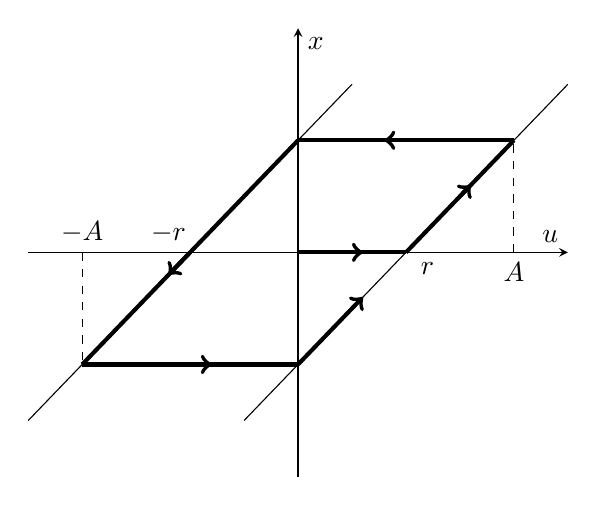
\begin{tikzpicture}
        \begin{axis} [
            xmin=-2.5, xmax=2.5, ymin=-2, ymax=2, 
            % grid=both,
            ylabel={$x$}, xlabel={$u$},
            % xtick={-2,-1.5,...,2}, ytick={-2,-1.5,...,2},
            % xticklabel style={font=\tiny, xshift=0.5ex},
            % yticklabel style={font=\tiny, yshift=0.5ex},
            axis line style={->},
            axis x line=middle,
            axis y line=middle,
            ticks=none
        ]
        \addplot+[solid, mark=none, color=black, domain=-2.5:0.5] {x+1};
        \addplot[line width=1.5pt, -> ,mark=none, color=black, domain=0:0.6] {0};
        \addplot[line width=1.5pt, - ,mark=none, color=black, domain=0.5:1] {0};

        \addplot[line width=1.5pt, -> ,mark=none, color=black, domain=1:1.6] {x-1};
        \addplot[line width=1.5pt, - ,mark=none, color=black, domain=1.5:2] {x-1};
        
        \addplot[line width=1.5pt, -> ,mark=none, color=black, domain=2:0.8] {1};
        \addplot[line width=1.5pt, - ,mark=none, color=black, domain=1:0] {1};
        
        \addplot[line width=1.5pt, -> ,mark=none, color=black, domain=0:-1.2] {x+1};
        \addplot[line width=1.5pt, - ,mark=none, color=black, domain=-1:-2] {x+1};
        
        \addplot[line width=1.5pt, -> ,mark=none, color=black, domain=-2:-0.8] {-1};
        \addplot[line width=1.5pt, - ,mark=none, color=black, domain=-1:0] {-1};
        
        \addplot[line width=1.5pt, -> ,mark=none, color=black, domain=0:0.6] {x-1};

        \node[below] at (1.2,0){$r$};
        \node[above] at (-1.2, 0){$-r$};
        \node[below] at (2,0) {$A$};
        \node[above] at (-2,0) {$-A$};
        \draw[dashed] (-2,0) -- (-2,-1);
        \draw[dashed] (2,0) -- (2,1);
        \addplot+[solid,mark=none, color=black, domain=-0.5:2.5] {x-1};
        
        \end{axis}
    \end{tikzpicture}

\end{document}